The focus is on the security aspects of autonomous on-road motor vehicles,
in particular the cybersecurity threats, standards, and industry practices used to secure these systems.
The focus will be on the current state of the VANETs communication main technologies and sensors of the perception systems,
analyzing the attack surface, main vulnerabilities and possible mitigations.

\subsection{Historical roots}\label{subsec:historical-roots}

The development of autonomous vehicles is a significant milestone in the evolution of intelligent transport systems.
It is important to start with some historical context to understand the current state of autonomous vehicles and then,
the security implications.

Vehicle automation has roots with General Motors showcasing the first concept of an automated vehicle in 1939.
Initial R\&D efforts were led by General Motors and the Radio Corporation of America Sarnoff Laboratory in the 1950s.
From 1964 to 2003, various government and academic initiatives in the US, Europe,
and Japan focused on automated buses, truck platoons, and advanced driving systems\cite{pendleton2017perception, shladover2017connected}.
A significant boost came from DARPA’s Grand Challenges Program in the 2000s\cite{darpa_grand_challenges_book},
where AVs first navigated desert terrains in 2005 and urban roads in 2007\cite{pendleton2017perception, shladover2017connected}.

Since then, researchers have rapidly progressed in academia and industry.
Volvo, Tesla, Audi, BMW,
Mercedes-Benz and Nissan are some of the major car manufacturers that have invested in AV technology\cite{faisal2019understanding}.

\begin{figure}[!htb]
    \centering
    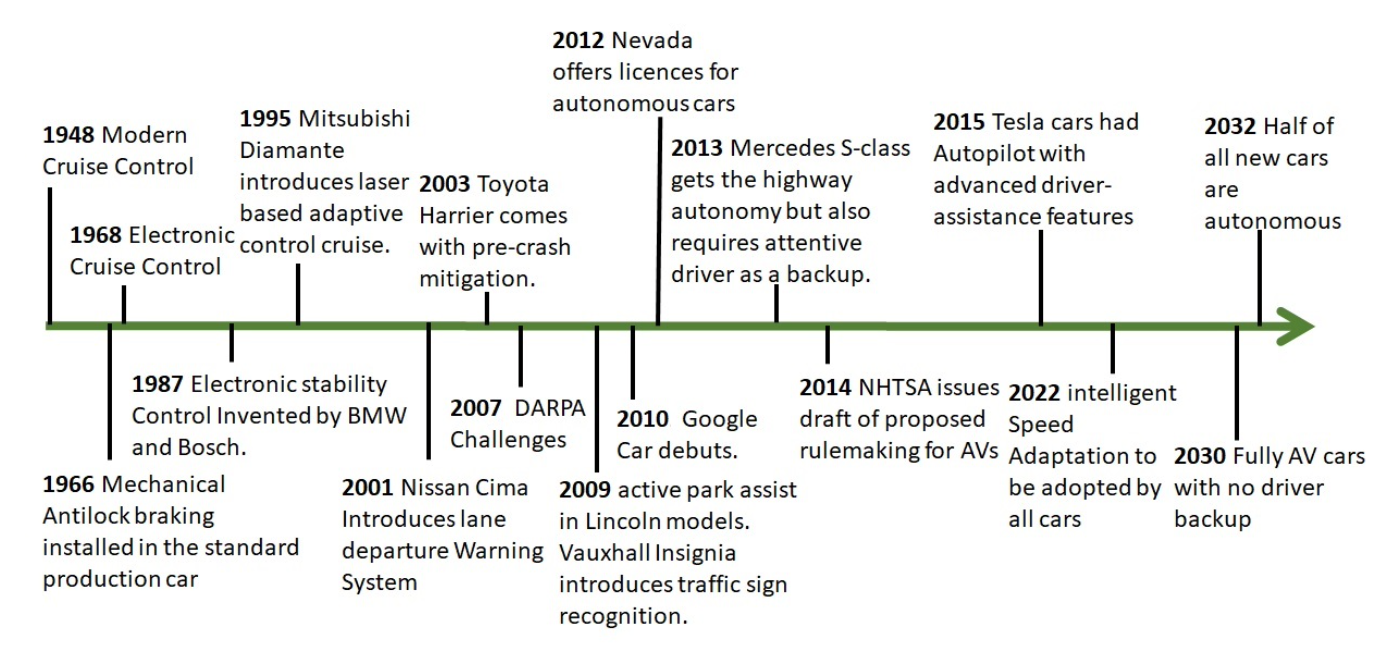
\includegraphics[width=0.7\linewidth]{figures/history}
    \caption{Historical timeline of autonomous vehicles.}
    \footnotesize{From \cite{ahangar2021survey} }
    \label{fig:history}
\end{figure}

\subsection{Autonomous Vehicles}\label{subsec:autonomous-vehicles}

The introduction on the market of autonomous vehicle brings to a revolutionary change in the automotive sector.
It is important to understand the impact that these vehicles can have on the society and the economy, influencing not only the automotive sector.
This type of vehicle can bring us to a new era of mobility, where transportation systems become intelligent, keeping in mind that connected components can be dangerous if not specially designed or well maintained\cite{schneier2014iot}

This major challenge, as often happens during times of innovation, has brought both advantages and drawbacks in terms of security.
What is intended is that the real driving force behind this innovation has been the convenience and socially beneficial aspects that have led to the rapid evolution of the sector.
However, as is often the case in such situations, some fundamental details get overlooked—it's a natural consequence.
In this instance, the principle of cybersecurity by design was overlooked\cite{sec-by-design}, and similar to the early development of the web, efforts are now underway to rectify this.

A lot of innovations also in terms of communication have been made since the introduction of these vehicles.
To improve functionalities, infotainment, safety, comfort and a lot of other aspects, vehicles require a lot of communication between them and the infrastructure like manufacturers backends or smart cities' services.
The shift from isolated and static systems to dynamic and interconnected systems increases the attack surfaces, particularly in terms of adaptability, dynamism, and awareness\cite{connected_vehicles_security_2023, bouchouia2023survey}.

For instance, vehicles relying on open software protocols and connecting with in-vehicle electric infrastructures play a vital role in strengthening their security framework.
With the need and integration of complex systems like the perception one, these vehicles essentially evolve into a highly sophisticated set of technologies influencing each other\cite{sec-by-design}.

\subsubsection{Levels of Automation}\label{subsubsec:levels-of-automation}
The level of driving automation is determined by the specific roles assigned to both the driving automation system feature and the human user in performing the dynamic driving task (DDT) and DDT fallback\cite{sae_j3016_2021}.
The manufacturer of the automation system defines the requirements, operational design domain (ODD), and operating characteristics of the feature, including its level of automation.
Additionally, the manufacturer outlines how the feature should be properly used, ensuring that its capabilities and limitations are clearly understood and followed during operation.
The Society of Automotive Engineers (SAE) has defined six levels of driving automation, ranging from no automation (Level 0) to full automation (Level 5)\cite{sae_j3016_2021}.

\begin{enumerate}
    \item \textbf{Level 0 (No Automation):} The human driver is responsible for all aspects of the dynamic driving task.
    \item \textbf{Level 1 (Driver Assistance):} The vehicle helps the driver with specific tasks, such as steering or acceleration (e.g.\ lane keeping assist, adaptive cruise control).
    \item \textbf{Level 2 (Partial Automation):} The vehicle can control both steering and acceleration/deceleration simultaneously under certain conditions, but the driver must remain engaged and monitor the environment (e.g. combined LKA and ADC in traffic conditions).
    \item \textbf{Level 3 (Conditional Automation):} The vehicle can perform all aspects of the DDT under certain conditions like in traffic jams or highway driving, but the driver must be ready to take over when prompted.
    \item \textbf{Level 4 (High Automation):} The user (become passenger) does not need to supervise the Automated driving system (ADS) or be receptive to a request to intervene while the
    ADS is engaged, restricted to some conditions (e.g., Google's Self-Driving Car\cite{teoh2017rage}).
    \item \textbf{Level 5 (Full Automation):} The vehicle can perform all aspects of the DDT under all conditions without human intervention.
\end{enumerate}

Levels 0–2 are generally classified as driver-assisted systems, while Levels 3 and 4 are considered semi-automated, and Level 5 represents full autonomy.

\begin{table}[ht]
    \centering
    \begin{tabular}{|c|l|}
        \hline
        \textbf{Acronym} & \textbf{Definition} \\ \hline
        ADS & Automated Driving System \\ \hline
        DDT & Dynamic Driving Task \\ \hline
        ODD & Operational Design Domain \\ \hline
        OEDR & Object and Event Detection and Response \\ \hline
    \end{tabular}
    \caption{Definitions of Key Acronyms in Automated Driving}
    \label{tab:acronyms}
\end{table}

\subsection{Overview of AVs Architecture}\label{subsec:overview-on-avs-architecture}

This section provides a high-level overview of the autonomous vehicles (AVs) architecture and the key parts that enable their operation.
Moreover, an alternative architecture proposed in\cite{ahangar2021survey} will be briefly discussed.
The architecture of AVs is designed to integrate various hardware and software components that work together to perceive the environment, make decisions, and control the vehicle\cite{architecture}.

\begin{figure}[!htb]
    \centering
    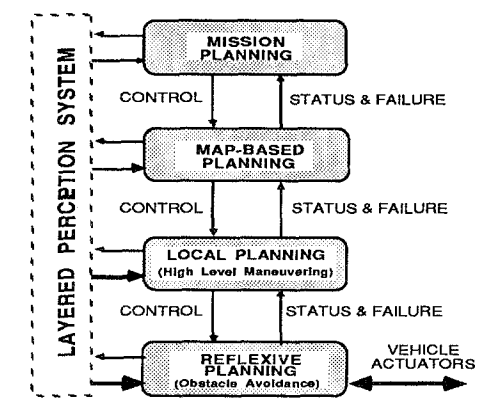
\includegraphics[width=0.7\linewidth]{figures/state-architecture}
    \caption{Hierarchical architecture of autonomous vehicles control.}
    \footnotesize{From \cite{architecture} }
    \label{fig:architecture}
\end{figure}

The overall architecture presented in\ref{fig:architecture} is composed of layers of hardware and software that interact to enable the vehicle to operate autonomously.
In its simplest and first form, the architecture consists of four main layers: perception, decision and planning, control and reflexive.
Each layer is responsible for a specific aspect of the AV's operation, from sensing the environment to executing driving maneuvers reflexively\cite{architecture}.

\begin{enumerate}
    \item \textbf{Perception}: This stage involves sensing the AV's surroundings using sensors.
    As expected, data processing is a fundamental step to exploit the correct information by other modules, such as adaptive detection and recognition frameworks, control systems, lane departure warning systems, traffic sign recognition, obstacle recognition, and vehicle positioning modules.
    The processed data is then sent to the decision and planning stage.
    It is important to note that performance in processing the data is fundamentals.
    \item \textbf{Decision and Planning}: Using the data from the perception stage, this stage plans and controls the AV's motion and behavior.
    It handles tasks like path planning, action prediction, and obstacle avoidance based on real-time maps, traffic data, user inputs, and past information.
    It may also include a data log module for error tracking and future reference.
    \item \textbf{Control}: The control module receives instructions from the decision and planning stage and manages the physical functions of the AV, such as steering, braking, and acceleration.
    \item \textbf{Reflexive}: This final stage interfaces with the mechanical components like the motors for the accelerator, brake, steering wheel, and gear.
    These components are controlled by the signals from the control module to execute the AV’s movements.
\end{enumerate}

The proposed and secured architecture extends this architecture providing four new layers: monitoring, analysis, decision-making, and visualization.
Any services, processes, and communication are monitored by the agents and analyzed by the process controllers.
A set of decision controllers act on the information from the process controllers.
The decisions are archived in a black box, while the analysis, reporting, and visualization layers are accessible both within the vehicle and through an external Virtual Security Operations Center (VSOC), allowing the user to consult them as needed\cite{adu-kyere2023self-aware}.

What can be easily noted is the need to monitor and analyze the data that are exchanged between the different components of the AVs.
Also, the data that are exchanged between the vehicle and the infrastructure should be monitored and analyzed to prevent and in case recover from possible attacks.
Some possible research directions could be the development of a secure and efficient monitoring system that can analyze the data in real-time and take action in case of attacks\ref{subsec:intrusion-detection-and-prevention-systems}.

\subsection{Social implications}\label{subsec:social-implications}

This section aims to provide a little insight into the social implications of autonomous vehicles.
The introduction of autonomous vehicles (AVs) is expected to have a profound impact on society\cite{thomas2020perception},
transforming transportation systems\cite{intelligent_transportation_2023}, urban planning\cite{impact_autonomous_vehicles_2018},
and the economy~\cite{economic_aspects_2020}.
Some potential pros and cons of AVs are summarized in Table~\ref{tab:table}.

\begin{table}[ht]
    \centering
    \begin{tabular}{|l|l|}
        \hline
        \textbf{Pros} & \textbf{Cons} \\ \hline
        Number of accidents reduced & Definition of legal responsibilities \\ \hline
        Time saved & Job losses \\ \hline
        Comfort & Price \\ \hline
    \end{tabular}
    \caption{Some pros and cons from \cite{ahangar2021survey} }\label{tab:table}
\end{table}

The consideration of time saved
is related to the trust that the user has in the vehicle and how effectively the cities in which the vehicles are used are designed and smart.

\subsection{Cyber-insecurity consequences}\label{subsec:cyber-insecurity}

Before introducing new threats of new autonomous vehicle technologies, it is important to understand some historical key attacks.
In the past, researchers have demonstrated various attacks on AVs, including remote hijacking, sensor spoofing, and data breaches.
The attack surface of AVs is expanding due to the increasing complexity of these systems, which rely on a combination of hardware, software, and communication technologies\cite{cybersec}.
This expansion is due to the aggressive attempts of manufacturers to
make vehicles fully autonomous in a short period of time and without considering the cybersecurity implications.
Focussing always on the functionalities offered to the driver in terms of comfort, the security of the vehicle has been considered as a secondary aspect, leading to a lot of vulnerabilities that can be exploited by attackers.

Some famous attacks that bring the attention to the cybersecurity of AVs are:
\begin{enumerate}
    \item The Jeep Cherokee hack in 2015: researchers remotely hijacked a Jeep Cherokee through its infotainment system, demonstrating the risks of cyber-attacks on connected vehicles\cite{miller2015remote}.
    \item The Tesla Model S hack in 2016: researchers exploited vulnerabilities in the vehicle's software to take control of the car's brakes, door locks, and other critical systems\cite{tesla_hack}.
    \item The Nissan Leaf hack in 2016: researchers demonstrated how an attacker could remotely control the vehicle's heating and air conditioning systems, drain the battery, and access the driver's personal information.
    \item The VW group hacked in 2016: researchers discovered vulnerabilities in the keyless entry systems of several VW group vehicles, allowing attackers to unlock the doors and start the engine without the key fob~\cite{garcia2016lock}.
    \item The Tesla cybertruck: it continues to be exploited by attackers to gain access to the vehicle's systems and control its functions remotely.
\end{enumerate}

These are only some examples of the risks associated with AVs and the need for robust cybersecurity measures to protect against cyber-attacks.